\documentclass[10pt]{extarticle}
\title{Analysis 2 Notes}
\author{Giacomo Ellero}
\date{Semester 2, 2023/2024}

\usepackage{amsfonts}
\usepackage{amsthm}
\usepackage{amssymb}
\usepackage{amsmath}
\usepackage{mathtools}
\usepackage{commath}
\usepackage{dirtytalk}
\usepackage{parskip}
\usepackage{mathrsfs}
\usepackage[many]{tcolorbox}
\usepackage{xparse}
\usepackage[a4paper,margin=1.5cm]{geometry}
\usepackage{bookmark}
\usepackage{physics}
\usepackage{tikz}
\usepackage{capt-of}
\usepackage{subfig}
\usepackage{cancel}

\newcommand{\C}{\mathbb{C}}
\newcommand{\R}{\mathbb{R}}
\newcommand{\F}{\mathcal{F}}
\renewcommand{\Re}{\operatorname{Re}}
\renewcommand{\Im}{\operatorname{Im}}

\newenvironment{absolutelynopagebreak}
  {\par\nobreak\vfil\penalty0\vfilneg
   \vtop\bgroup}
  {\par\xdef\tpd{\the\prevdepth}\egroup
   \prevdepth=\tpd}

\newtcolorbox{examplebox}[1]{colback=green!5!white,colframe=green!40!black,title={#1},fonttitle=\bfseries,parbox=false}
\newtcolorbox{notebox}[1]{colback=blue!5!white,colframe=blue!40!black,title={Note: #1},fonttitle=\bfseries,parbox=false}
\newtcolorbox{bluebox}[1]{colback=blue!5!white,colframe=blue!40!black,title={#1},fonttitle=\bfseries,parbox=false}
\newtcolorbox{warningbox}[1]{colback=orange!5!white,colframe=orange!90!black,title={Warning: #1},fonttitle=\bfseries,parbox=false}
   
\begin{document}

\maketitle
\tableofcontents
\clearpage

\section{Class of 12/02/2024}

In this class we will discuss mainly multivariable calculus:
\begin{itemize}
    \item Parametric curves: $\R \to \R^d$.
    \item Graphs: $\R^2 \to \R$.
    \item Vector fields: $\R^d \to \R^d$.
\end{itemize}

And in general we will discuss functions $f: \R^d \to \R^p$.

$\R^d$ is a vector space, like the ones we have seen in linear algebra, so many notions carry over.

\subsection{Dot product and distance}

\textbf{\underline{Definition} (dot product)}: Let $x, y \in \R^d$. The dot product of $x$ and $y$ is defined as

$$
    \underline{x} \cdot \underline{y} = \sum_{i=1}^d x_i y_i
$$

We have seen dot products (inner products) in linear algebra but we will see some of their proprieties again:
\begin{enumerate}
    \item $\underline{x} \cdot \underline{y} = \underline{y} \cdot \underline{x}$.
    \item $\underline{x} \cdot (\underline{y} + \underline{z}) = \underline{x} \cdot \underline{y} + \underline{x} \cdot \underline{z}$.
    \item $\underline{x} \cdot \underline{x} \geq 0$ and $\underline{x} \cdot \underline{x} = 0 \iff \underline{x} = \underline{0}$.
\end{enumerate}

\subsubsection{Norm}

\textbf{\underline{Definition} (norm)}: Let $\underline{x} \in \R^d$. The norm of $\underline{x}$ is defined as

$$
    \norm{\underline{x}} = \sqrt{\underline{x} \cdot \underline{x}}
$$

For a more general definition see the linear algebra notes.

\subsection{Cauchy-Schwarz inequality}

\textbf{\underline{Theorem} (Cauchy-Schwarz inequality)}: Let $\underline{x}, \underline{y} \in \R^d$. Then

$$
    \abs{\underline{x} \cdot \underline{y}} \leq \norm{\underline{x}} \norm{\underline{y}}
$$

\begin{proof}
    We introduce $f(t) = \norm{\underline{x} + t \underline{y}}^2$.

    We apply some algebraic manipulation to $f(t)$ according to the proprieties of the dot product and the norm:

    \begin{align*}
        f(t) & = \norm{\underline{x} + t \underline{y}}^2                                                                                                              \\
             & = (\underline{x} + t \underline{y}) \cdot (\underline{x} + t \underline{y})                                                                             \\
             & = \underline{x} \cdot (\underline{x} + t \underline{y}) + t \underline{y} \cdot (\underline{x} + t \underline{y})                                       \\
             & = \underline{x} \cdot \underline{x} + t \underline{x} \cdot \underline{y} + t \underline{y} \cdot \underline{x} + t^2 \underline{y} \cdot \underline{y} \\
             & = \norm{\underline{x}}^2 + 2t \underline{x} \cdot \underline{y} + t^2 \norm{\underline{y}}^2
    \end{align*}

    If $\underline{y} \ne 0$ we have that $f(t)$ is a parabola which is always positive, hence $\Delta \leq 0$. We have

    \begin{align*}
        \Delta & = (2 \underline{x} \cdot \underline{y})^2 - 4 \norm{\underline{x}}^2 \norm{\underline{y}}^2        \\
               & = 4 (\underline{x} \cdot \underline{y})^2 - 4 \norm{\underline{x}}^2 \norm{\underline{y}}^2 \leq 0 \\
    \end{align*}

    We pass to the inequality and we get

    \begin{align*}
        \cancel{4}(\underline{x} \cdot \underline{y})^2 & \leq \cancel{4} \norm{\underline{x}}^2 \norm{\underline{y}}^2 \\
        \abs{\underline{x} \cdot \underline{y}} ^2      & \leq \norm{\underline{x}}^2 \norm{\underline{y}}^2            \\
        \abs{\underline{x} \cdot \underline{y}}         & \leq \norm{\underline{x}} \norm{\underline{y}}
    \end{align*}
\end{proof}

Note that if $\Delta = 0$ it's easy to prove that $\underline{x}$  = t $\underline{y}$, hence they are linearly dependent. This is the only case in which the inequality becomes an equality.

\subsection{Defining the angle between two vectors}

\textbf{\underline{Definition} (angle)}: Let $\underline{x}, \underline{y} \in \R^d$. The following relation holds between the dot product and the angle $\theta$ between the two vectors:

$$
    \underline{x} \cdot \underline{y} = \norm{\underline{x}} \norm{\underline{y}} \cos \theta
$$

hence

$$
    \theta = \arccos \left( \frac{\underline{x} \cdot \underline{y}}{\norm{\underline{x}} \norm{\underline{y}}} \right)
$$

From the definition we get that $\underline{x} \cdot \underline{y} = 0 \iff \theta = \frac{\pi}{2}$.

Cauchy-Schwarz inequality guarantees that the argument of $\arccos$ is always between -1 and 1.

Note that this is a definition, not a theorem: we are defining the concept of angle from the dot product.

\section{Class of 14/02/2024}

These theorems have been covered already in linear algebra, see the notes for more details.

\subsection{Triangle inequality}

\textbf{\underline{Theorem} (triangle inequality)}: Let $\underline{x}, \underline{y} \in \R^d$. Then

$$
    \norm{\underline{x} + \underline{y}} \leq \norm{\underline{x}} + \norm{\underline{y}}
$$

\begin{proof}
    We have that

    \begin{align*}
        \norm{\underline{x} + \underline{y}}^2 & = (\underline{x} + \underline{y}) \cdot (\underline{x} + \underline{y})                                                                         \\
                                               & = \underline{x} \cdot (\underline{x} + \underline{y}) + \underline{y} \cdot (\underline{x} + \underline{y})                                     \\
                                               & = \underline{x} \cdot \underline{x} + \underline{x} \cdot \underline{y} + \underline{y} \cdot \underline{x} + \underline{y} \cdot \underline{y} \\
                                               & = \norm{\underline{x}}^2 + 2 \underline{x} \cdot \underline{y} + \norm{\underline{y}}^2
    \end{align*}

    We apply the Cauchy-Schwarz inequality and we get

    \begin{align*}
        \norm{\underline{x} + \underline{y}}^2 & \leq \norm{\underline{x}}^2 + 2 \norm{\underline{x}} \norm{\underline{y}} + \norm{\underline{y}}^2 \\
        \norm{\underline{x} + \underline{y}}^2 & \leq \left(\norm{\underline{x}} + \norm{\underline{y}}\right)^2
    \end{align*}

    We take the square root of both sides and we get the result.
\end{proof}

\subsection{Pythagorean theorem}

\textbf{\underline{Theorem} (Pythagorean theorem)}: Let $\underline{x}, \underline{y} \in \R^d$ be orthogonal. Then

$$
    \norm{\underline{x} + \underline{y}}^2 = \norm{\underline{x}}^2 + \norm{\underline{y}}^2
$$

I will not report the proof here, if you're interested you can find it in my linear algebra notes.

\subsection{Law of cosines}

This is a generalization of the Pythagorean theorem.

\textbf{\underline{Theorem} (law of cosines)}: Let $\underline{x}, \underline{y} \in \R^d$. Then

$$
    \norm{\underline{x} - \underline{y}}^2 = \norm{\underline{x}}^2 + \norm{\underline{y}}^2 - 2 \norm{\underline{x}} \norm{\underline{y}} \cos \theta
$$

where $\theta$ is the angle between $\underline{x}$ and $\underline{y}$.

\subsection{Planes}

Planes in $\R^3$ are identified by a point $A$ and a normal vector $\underline{n}$.

A point $M = \begin{pmatrix}
        x \\ y \\ z
    \end{pmatrix} \in \R^3$ belongs to a plane $\pi$ if and only if the vector $AM$ is orthogonal to $\underline{n}$.

This means that the equation of the plane is

$$
    \left(
    \begin{pmatrix}
            x \\ y \\ z
        \end{pmatrix} - \begin{pmatrix}
            A_x \\ A_y \\ A_z
        \end{pmatrix}
    \right)
    \cdot
    \begin{pmatrix}
        n_x \\ n_y \\ n_z
    \end{pmatrix}
    = 0
$$

\subsection{Orientation of vectors}

Consider $B_1, B_2$ be pairs of vectors in $\R^2$.

\begin{center}
    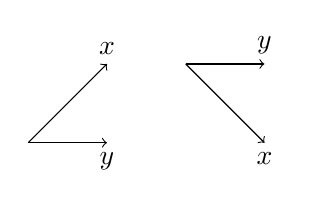
\begin{tikzpicture}
        \draw[->] (-1, 0) -- (0, 1) node[anchor=south] {$x$};
        \draw[->] (-1, 0) -- (0, 0) node[anchor=north] {$y$};

        \draw[->] (1, 1) -- (2, 1) node[anchor=south] {$y$};
        \draw[->] (1, 1) -- (2, 0) node[anchor=north] {$x$};
    \end{tikzpicture}

    \captionof{figure}{Two pair of vectors $B_1$ and $B_2$}
    \label{fig:orientation_of_vectors}
\end{center}

$B_1$ and $B_2$ are both bases of $\R^2$, but if we try to \say{continuously} transform one into the other by \say{rotating} the vectors
while keeping them a basis we will see that at some point we will have $\underline{x} \cdot \underline{y} = 0$,
hence the two vectors no longe form a basis.

We call this propriety the \textbf{orientation} of the basis.
When we choose the orientation of the axis of a space we are choosing the orientation of the basis.

By convention we say that the positive orientation of the basis is the one defined by the right-hand rule.

We can extend this concept to $\R^d$ by considering the determinant of the matrix of the vectors.

\subsection{Determinant}

Determinants have been covered already in linear algebra, for definition and proprieties see those notes.
We will discuss here some of their geometric proprieties that weren't covered before.

In $\R^2$ the determinant of a matrix of two vectors is the area of the parallelogram defined by the two vectors.
In $\R^3$ it is the volume of the parallelepiped defined by the three vectors.

\begin{gather*}
    \det \left( \begin{pmatrix}
            \underline{x} & \underline{y}
        \end{pmatrix} \right) = \text{ area} \\
    \det \left( \begin{pmatrix}
            \underline{x} & \underline{y} & \underline{z}
        \end{pmatrix} \right) = \text{ volume}
\end{gather*}

\subsubsection{Cross product}

\textbf{\underline{Definition} (cross product)}: Let $\underline{x} = \begin{pmatrix}
        x_1 \\ x_2 \\ x_3
    \end{pmatrix}$ and $\underline{y} = \begin{pmatrix}
        y_1 \\ y_2 \\ y_3
    \end{pmatrix}$.
The cross product of $\underline{x}$ and $\underline{y}$ is the vector

$$
    \underline{x} \times \underline{y} = \begin{pmatrix}
        x_2 y_3 - x_3 y_2 \\
        x_3 y_1 - x_1 y_3 \\
        x_1 y_2 - x_2 y_1
    \end{pmatrix}
$$

\subsubsection{Cross product and determinant}

\textbf{\underline{Theorem}}: Let $\underline{x}, \underline{y}, \underline{z} \in \R^3$. Then

$$
    \det \left( \begin{pmatrix}
            \underline{x} & \underline{y} & \underline{z}
        \end{pmatrix} \right) = (\underline{x} \times \underline{y}) \cdot \underline{z}
$$

\begin{proof}
    We have that

    \begin{align*}
        \det \left( \begin{pmatrix}
                            \underline{x} & \underline{y} & \underline{z}
                        \end{pmatrix} \right)
         & = \det \begin{pmatrix}
                      x_1 & y_1 & z_1 \\
                      x_2 & y_2 & z_2 \\
                      x_3 & y_3 & z_3
                  \end{pmatrix}                                                        \\
         & = z_1 \det \begin{pmatrix}
                          x_2 & y_2 \\
                          x_3 & y_3
                      \end{pmatrix}
        - z_2 \det \begin{pmatrix}
                       x_1 & y_1 \\
                       x_3 & y_3
                   \end{pmatrix}
        + z_3 \det \begin{pmatrix}
                       x_1 & y_1 \\
                       x_2 & y_2
                   \end{pmatrix}                                                        \\
         & = z_1 (x_2 y_3 - x_3 y_2) - z_2 (x_1 y_3 - x_3 y_1) + z_3 (x_1 y_2 - x_2 y_1) \\
         & = \begin{pmatrix}
                 z_1 \\ z_2 \\ z_3
             \end{pmatrix} \cdot (\underline{x} \times \underline{y})
    \end{align*}

    The last steps follow from the definition of determinant for $2 \times 2$ matrixes and the definition of the cross product.
\end{proof}


% TODO: add previous classes

\section{Class of 16/02/2024}

\subsection{Parametrizing ellipses}

Last class we saw how to parametrize lines and circles, now we will have a look at ellipses.

An ellipse is defined by the parametrization

\[
    \begin{cases}
        x = a \cos t \\
        y = b \sin t
    \end{cases}
\]

where $a$ and $b$ are the semi-axes of the ellipse. Note that if $a = b$ we get a circle of radius $a$.

For the equation we have

$$
    \frac{x^2}{a^2} + \frac{y^2}{b^2} = 1
$$

The ellipse is the image of the unit circle by tge linear transformation $\begin{pmatrix}
        x \\ y
    \end{pmatrix} \to \begin{pmatrix}
        ax \\ by
    \end{pmatrix}$.

\subsubsection{Applying transformations to curves}

Consider curve $\gamma_1$ which we want to rotate by an angle $\theta$ to obtain $\gamma_2$.

Remember the rotation matrix

$$
    R(\theta) = \begin{pmatrix}
        \cos \theta & -\sin \theta \\
        \sin \theta & \cos \theta
    \end{pmatrix}
$$

For the parametrization is quite easy since we just need to multiply the vector by the rotation matrix.

$$
    \begin{pmatrix}
        x \\ y
    \end{pmatrix} = \begin{pmatrix}
        \cos \theta & -\sin \theta \\
        \sin \theta & \cos \theta
    \end{pmatrix} \begin{pmatrix}
        f(t) \\ g(t)
    \end{pmatrix}
$$

Getting the equation is a bit trickier.
We have to invert the transformation matrix:
consider a point $(x, y)$ on $\gamma_2$, we have that $(x, y) = R(\theta) (x', y')$, hence $(x', y') \in \gamma_1 = R(-\theta) (x, y)$.
We have that $(x,y) \in \gamma_2 \iff R(-\theta)(x, y) \in \gamma_1$.
Now we have $(x', y')$ in terms of $(x, y)$ and we can plug the result of the reverse transformation into the equation of $\gamma_1$.

\subsection{Cylinders}

Let $(x, y, z) \in \R^3$. We have that $\sqrt{x^2 + y^2 + z^2}$ is the distance from the origin and $\sqrt{x^2 + y^2}$ is the distance to the $Oz$ axis.

The equation of a cylinder is

$$
    \left\{ (x, y, z) \in \R^3  : x^2 + y^2 = r^2\right\}
$$

we are basically saying that the distance from the $Oz$ axis is constant and is equal to $r$.

\subsection{Cones}

The way we describe cones is by saying that if we slice the cone at altitude $z$ we will have a circle of radius $z$ and center at $(0,0,z)$.

So we want $\sqrt{x^2 + y^2} = |z|$, hence

$$
    \left\{ (x, y, z) \in \R^3 : x^2 + y^2 = z^2 \right\}
$$

\subsubsection{Variations of the cone}

We can consider the following variations

$$
    x^2 + y^2 = z^2 + 1 \\
    x^2 + y^2 = z^2 - 1
$$

In the first one we have that at $z=0$ we have a circle of radius 1, in the second one we have that at $z=0$ we have a circle of radius $-1$ which is not possible, hence the second equation only gets to $z = \pm 1$.

These type of surfaces are called hyperboloids of revolution.

% TODO: Add the drawings

\subsection{Parametric curves}

We can now give a formal definition of a parametric curve.

\underline{Definition}: A parametric curve $\gamma$ is a function of $t \in I \subseteq \R$ and valued in $\R^d$.

$$
    \gamma(t) = \begin{pmatrix}
        \gamma_1(t) \\
        \vdots      \\
        \gamma_d(t)
    \end{pmatrix} \in \R^d
$$

where $\gamma_1, \ldots, \gamma_d$ are the coordinate functions defined as $\gamma_i: I \to \R$.

Parametric curves are basically the description of the motion of a point in space as a function of time.

\underline{Definition}: The \textbf{domain of definition} of $\gamma$ is the intersection of the domains of the coordinate functions.

\subsubsection{How to represent a curve}

There are many ways to represent a curve, for example we could graph the individual coordinate functions but this is not very representative of the curve itself.

We can try to use a graph to represent a curve $\gamma$:

\underline{Definition}: The \textbf{graph} of $\gamma$ is the subset of $\R^{d+1}$ made of points
$$
    (t, \gamma(t)) = (t, \gamma_1(t), \ldots, \gamma_d(t))
$$
for $t \in I$.

The graphs contains all the information about the curve, but it is not very practical to use because of its complexity.

\underline{Definition}: The \textbf{image} of $\gamma$ is the subset of $\R^d$ made of points $\gamma(t)$ for $t \in I$.

The image is basically the graphs seen from the $x$ axis.

This representation is quite practical but we are losing some information about the parameter $t$, this is mostly ok though.

Note that different curves will always have different graphs but might have the same image.

\underline{Remark}: Every graph is the image of some function in $\R^{d+1}$, but not all images are graphs of some function in $\R^{d-1}$.

\section{Class of 19/02/2024}

\subsection{Continuity and differentiability for parametric curves}

\textbf{\underline{Definition} (continuity)}: Let $\gamma: t \to (\gamma_1, \gamma_2, \ldots, \gamma_d) \in R^d$ be a parametric curve.
$\gamma$ is continuous at $t_0 \in I$ if all the functions $\gamma_1, \ldots, \gamma_d$ are continuous at $t_0$.

\textbf{\underline{Definition} (differentiability)}: Let $\gamma: t \to (\gamma_1, \gamma_2, \ldots, \gamma_d) \in R^d$ be a parametric curve.
$\gamma$ is differentiable at $t_0 \in I$ if all the functions $\gamma_1, \ldots, \gamma_d$ are differentiable at $t_0$.
We define $\gamma'(t_0) = (\gamma_1'(t_0), \ldots, \gamma_d'(t_0))$.

\textbf{\underline{Definition} (speed)}: Let $\gamma: t \to (\gamma_1, \gamma_2, \ldots, \gamma_d) \in R^d$ be a parametric curve differentiable at $t_0 \in I$.
Its speed at $t_0$ is $\norm{\gamma'(t_0)}$.

\underline{Example}: consider the unit circle $\gamma(t) = (\cos t, \sin t)$, we have that

$$
    \gamma'(t) = (-\sin t, \cos t)
$$

and
$$
    \norm{\gamma'(t)} = \sqrt{(-\sin t)^2 + \cos^2 t} = 1
$$

\textbf{\underline{Definition} (higher order differentiability)}:
The parametric curve $\gamma$ is $k$ times differentiable at $t_0 \in I$ if all the functions $\gamma_1, \ldots, \gamma_d$ are $k$ times differentiable at $t_0$.

Note that in physics we sometimes use $\dot{o}, \ddot{o}, \ldots$ to denote the derivative of a function with respect to time.

\subsection{Taylor expansion and local behavior}

\textbf{\underline{Definition} (regular point)}:
If $\gamma: I \to \R^d$ is differentiable at $t_0 \in I$, we say that $t_0$ is a regular point if $\gamma'(t_0) \neq \underline{0}$.

\textbf{\underline{Definition} (tangent line)}:
If $\gamma$ is differentiable and $t_0$ is a regular point, the tangent to the image of $\gamma$ at $\gamma(t_0)$ is the line passing through $\gamma(t_0)$ and directed by $\gamma'(t_0)$.
That is

$$
    h \in R \mapsto \gamma(t_0) + h \gamma'(t_0) \in \R^d
$$

\subsubsection{Equation of a line}

We can write the equation of a line from a point and a normal vector:

$$
    \left(
    \begin{pmatrix}
            x \\ y
        \end{pmatrix} - \begin{pmatrix}
            x_0 \\ y_0
        \end{pmatrix}
    \right) \cdot \begin{pmatrix}
        a \\ b
    \end{pmatrix} = 0
$$

where $\begin{pmatrix}
        a \\ b
    \end{pmatrix}$ is the normal vector to the line and $\begin{pmatrix}
        x_0 \\ y_0
    \end{pmatrix}$ is a point on the line.


\underline{Example} (unit circle):
Consider the tangent on the unit circle. We have that its parametrization is
$$
    h \mapsto \begin{pmatrix}
        \cos t_0 \\ \sin t_0
    \end{pmatrix} + h \begin{pmatrix}
        -\sin t_0 \\ \cos t_0
    \end{pmatrix} =
    \begin{pmatrix}
        \cos t_0 - h \sin t_0 \\
        \sin t_0 + h \cos t_0
    \end{pmatrix}
$$

In the case of the unit circle the normal vector is

$$
    \begin{pmatrix}
        a \\ b
    \end{pmatrix}
    =
    \begin{pmatrix}
        -\cos t_0 \\ -\sin t_0
    \end{pmatrix}
    =
    - \gamma(t_0)
$$

(Note that this is the case only for the unit circle.)

We have that the equation of the tangent line of the unit circle at $t_0$ is

$$
    \left(
    \begin{pmatrix}
            x \\ y
        \end{pmatrix} - \begin{pmatrix}
            \cos t_0 \\ \sin t_0
        \end{pmatrix}
    \right)
    \cdot
    \begin{pmatrix}
        -\cos t_0 \\ -\sin t_0
    \end{pmatrix}
    = 0
$$

\underline{Example} ($t_0$ is not a regular point):
Let $\gamma(t) = (t^2, t^3)$, which is continuous and differentiable.
Let $t_0 = 0$, we that $\gamma'(t_0) = \underline 0$.
We have that
$$
    \begin{cases}
        y = x^{3/2}  & \text{ if } t \geq 0 \\
        y = -x^{3/2} & \text{ if } t \leq 0
    \end{cases}
$$

with $x \geq 0$. We see how $\gamma'(t_0)$ exists but is not regular.

We call this an \textbf{ordinary cusp} (formal definition later).

\begin{figure}
    \centering
    \subfloat[\centering Image]{{
                \includegraphics[width=0.35\textwidth]{assets/ordinary_cusp_image.png}
            }}
    \subfloat[\centering Graph]{{
                \includegraphics[width=0.35\textwidth]{assets/ordinary_cusp_graph.png}
            }}
    \caption{Ordinary cusp}
    \label{fig:ordinary_cusp}
\end{figure}

\subsubsection{Taylor expansion}

\textbf{\underline{Definition} (Taylor expansion)}:
Let $\gamma: I \to \R^d$ be $k$ times differentiable over $I$.
Then

$$
    \gamma(t_0 + h) =
    \gamma(t_0) +
    h \gamma'(t_0) +
    \frac{h^2}{2!} \gamma''(t_0) +
    \ldots +
    \frac{h^k}{k!} \gamma^{(k)}(t_0) +
    o(h^k)
$$

From this definition we see that the image of $\gamma$ is close to $\gamma (t_0)$ since it is the principal term of the expansion.

Moreover note that the Taylor expansion of order 1 with $\gamma'(t_0) \ne \underline 0$ is

$$
    \gamma(t_0 + h) = \gamma(t_0) + h \gamma'(t_0) + o(h)
$$

which is the equation of the tangent line.

\subsubsection{Local behavior}

We can use the Taylor expansion to study the behavior of a curve in the neighborhood of $t_0$.

% TODO: add graphs

\textbf{\underline{Definition} (biregular point)}:
Let $\gamma: I \to \R^d$ such that $\gamma'(t_0) \ne \underline 0$ and $\gamma''(t_0)$ is linearly independent from $\gamma'(t_0)$.
Then we say that $t_0$ is a biregular point.

\textbf{\underline{Definition} (inflection point)}:
$t_0$ is an inflection point if $\gamma'(t_0) \ne \underline 0$ but $\gamma''(t_0)$ is linearly dependent from $\gamma'(t_0)$.

This means that the curve crosses the tangent line at $t_0$.


\textbf{\underline{Definition} (ordinary cusp)}:
$t_0$ is an ordinary cusp if $\gamma'(t_0) = \underline 0$ but $\gamma''(t_0), \gamma'''(t_0)$ are linearly independent.

\begin{figure}
    \centering
    \subfloat[\centering Inflection point]{{
                \includegraphics[width=0.35\textwidth]{assets/inflection_point.png}
            }}
    \subfloat[\centering Ordinary cusp]{{
                \includegraphics[width=0.35\textwidth]{assets/ordinary_cusp.png}
            }}
    \caption{Inflection point and ordinary cusp}
    \label{fig:inflection_point_and_ordinary_cusp}
\end{figure}


\end{document}